\documentclass[12pt,a4paper]{article}
\usepackage[utf8]{inputenc}
\usepackage[spanish]{babel}


% Paquetes

\usepackage{amsmath}
\usepackage{amsfonts}
\usepackage{amssymb}
\usepackage{amsthm}  % Permite crear teoremas nuevos / Estilos de teoremas 
\usepackage{graphicx} % 
\usepackage[colorlinks=true,allcolors=blue]{hyperref} % Crea las hiperreferencias (clicas y te mueves)
\graphicspath{ {Imagenes/} }
\usepackage{fancybox} % para usar la caja de los ejemplos
\usepackage{bigints } % permite crear grandes integrales
% Autor y titulo

\title{Apuntes Mecánica Estadística}
\author{Daniel Vázquez Lago}

% Forma del  texto

\setlength{\parindent}{15px}
\usepackage[left=2.25cm,right=2cm,top=4cm,bottom=2cm]{geometry}

% Otros


\numberwithin{equation}{section}
\numberwithin{figure}{section}

% Comandos propios
\newcommand{\tquad}{\quad \quad \quad}

\newcommand{\parentesis}[1]{\left( #1  \right)}
\newcommand{\parciales}[2]{\frac{\partial #1}{\partial #2}}
\newcommand{\pparciales}[2]{\parentesis{\parciales{#1}{#2}}}
\newcommand{\dparciales}[2]{\dfrac{\partial #1}{\partial #2}}
\newcommand{\ccorchetes}[1]{\left[ #1  \right]}
\newcommand{\D}{\mathrm{d}}
\newcommand{\derivadas}[2]{\frac{\D #1}{\D #2}}
\newcommand{\cte}{\mathrm{cte}}

\newcommand{\estado}[1]{| \Psi_{ #1} \rangle}


\newcommand{\eup}{\mid \uparrow \rangle}
\newcommand{\edw}{\mid \downarrow \rangle}

% Comandos vectoriales

\newcommand{\kn}{\mathbf{k}}
\newcommand{\pn}{\mathbf{p}}
\newcommand{\qn}{\mathbf{q}}
\newcommand{\rn}{\mathbf{r}}
\newcommand{\un}{\mathbf{u}}
\newcommand{\vn}{\mathbf{v}}
\newcommand{\xn}{\mathbf{x}}


\newcommand{\An}{\mathbf{A}}
\newcommand{\Pn}{\mathbf{P}}
\newcommand{\Jn}{\mathbf{J}}

\newcommand{\Sigman}{\boldsymbol{\Sigma}}

% Comandos vectoriales unitarios

\newcommand{\hrho}{\hat{\rho}}

% Comandos teoremas

\newtheorem{theorem}{Teorema}[section]
\newtheorem{principio}{Principio}[section]
\newtheorem{corollary}{Corolario}[theorem]
\newtheorem{lemma}{Lema}[section]
\newtheorem{ejemplo}{Ejemplo}[section]

\theoremstyle{definition}
\newtheorem{definition}{Definicion}[section]

\begin{document}

\maketitle

\newpage

\tableofcontents

\newpage

\section{Fundamentos de la Mecánica Estadística}

\subsection{Microestado y Macroestado}

La descripción del estado del sistema desde la perspectiva macroscópia se realiza en términos de parámetros fenomenológicos como presión, temperatura, composición química... Esto es, en término de variables de estado del sistema globalmente considerado y en funciones de las mismas. Los estados así descritos reciben el nombre de \textbf{macroestados}. \\

No obstante, el sistema está compuesto por constituyentes microscópicos, y es posible optar por una descripción microscópica de su estados especificando el estado mecánico de todos sus constituyentes, bien mediante la mecánica clásica o especificando el estado cuántico de todos ellos. El resultado así obtenido se denomina microestado del sistema, y obviamente tiene una cantidad de información mucho mayor que la correspondiente al macroestado. Desde esta perspectiva, definimos \textbf{microestado} como cualquier configuración microscópica que el sistema pueda adoptar en el curso de sus fluctuaciones microscópicas y, aunque cambia con una frecuencia elevada, el macroestado del sistema no lo hace, por lo que debemos concluir que cada macroestado es compatible con un número muy elevado de microestados. \\

El hecho fundamental de la Mecánica Estadística es que los microestados del sistema deben ser tratados como sucesos aleatorios al no disponer información incompleta de ellos, bien por su imposiblidad práctica en la mecánica clásica o su imposibilidad conceptual en la mecánica cuántica. 

\subsection{Volumen fásico y densidad de estados}

La pregunta que nos atañe ahora es, ¿Cuantos microestados son compatibles con una cofiguración macroscópica dada? Evidentemente la respuesta será diferente en función del lenguaje con el que describamos el problema (mecánica cuántica o mecánica clásica). Primero tratemos de resolver el problema en la mecánica clásica para luego generalizar el problema a la mecánica cuántica. \\

Para poder responder a la pregunta primero tenemos que definir el \textit{espacio fásico} o \textit{espacio de fases}, que denotaremos por $\Gamma$. Sea un sistema formado por $N$ partículas con $f$ grados de libertad. Para describir el estado de una sola partícula debemos conocer $2f$ coordenadas ($f$ posiciones y $f$ momentos). Para describir el estado de las $N$ partículas necesitaremos entonces $2Nf$ coordenadas, que denotaremos por $(\pn^N,\qn^N)$. Es evidente que \textit{cualquier microestado} estará completamente determinado por estas coordenadas. Conocer un microestado implica conocer dichas coordenadas. \\

Es decir, cada microestado tiene definida una posición en el espacio fásico. Si $R$ es una región del espacio fásico, limitada por una hiper-superficie, podemos definir el \textbf{volumen fásico} de dicha región como:

\begin{equation}
\Gamma  = \bigintssss_R \prod^N_{i=1} \D \qn_i \D \pn_i
\end{equation}
donde la hipersuperficie viene determinada por una o varias restricciones o ligaduras. Definamos como $\D \Gamma$ a:

\begin{equation}
\D \Gamma  \equiv \prod_{i=1}^N \D \pn_i \D \qn_i
\end{equation}
Ahora evaluemos el volumen fásico definido por una hiper-superficie de energía constante $H(\qn^N,\pn^N)=E$. Está claro que todo punto del espacio de fases dentro de ese volumen verificará que $H (\qn^N,\pn^N ) \leq  E$. Entonces el volumen del espacio de fases:
\begin{equation}
\Gamma = \bigintssss \theta\ccorchetes{E-H\parentesis{\qn^N,\pn^N}} \D \Gamma
\end{equation}
donde $\theta[E-H]$ es la \textit{función de Heavside}. Como hemos dicho anteriormente, conocer el microestado de un sistema es equivalente a conocer todas las coordenadas. Entonces podemos ver al volumen fásico como el \textit{número de estados compatibles con una determinada restricción}. En el caso visto ahora la restricción es $H=E$. A partir de esta magnitud es inmediato obtener el número de estados que tienen una determinada energía $E$, que será la diferencia entre los estados con energía $E$ y $E+\D E$. \\

Una vez hemos entendido la relación volumen fásico-número de estados, podemos definir a partir de esta magnitud la \textbf{densidad de estados} $g(E)$ por intervalo de energía, tal que

\begin{equation}
g(E) = \derivadas{\Gamma(E)}{E}
\end{equation}
que como podemos ver es básicamente el número de estados que le corresponden una determinada energía, ya que si $\delta$ es la \textit{función delta de Dirac}:

\begin{equation}
g(E) = \int \delta \ccorchetes{E-H\parentesis{\qn^N,\pn^N}} \D \Gamma
\end{equation}
es decir, $g(E)$ es el \textit{número de estados compatibles con una energía dada}. También se le denomina \textit{degeneración}, por razones que ya veremos más adelante. \\

Como podemos ver ya somos capaces de calcular el número de estados compatibles con un sistema: solo hay que aplicar una o varias restricciones al espacio de fases e integrar. Luego si queremos calcular el número de estados para una energía constante... bastaría con derivar dicho volumen. A pesar de todo lo comentando, los resultados desde una perspectiva dimensional no tienen sentido. El número de estados es una cantidad adimensional, y sin embargo tiene unidades de acción (unidades de acción elevada a $Nf$). \\

Para arreglar esto lo que podemos hacer es dividir por una constante $h^{Nf}$ con unidades de acción. Esto es lo mismo que suponer que el volumen fásico está dividido en pequeños volúmenes de tamaño $h^{Nf}$ tal que cada uno de estos implica un estado. Esto es análogo a ``cuantizar'' el volumen fásico. De hecho si siguiéramos este mismo proceso (calcular el volumen fásico, relacionarlo con el número de estados...) pero ahora usando la mecánica cuántica, obtendríamos el mismo resultado pero con este $h$ siendo la \textit{constante de Plank}, que de hecho tiene unidades de acción. Usar la física cuántica es la solución natural a nuestro problema. La cuantización tiene su naturaleza en el principio de incertidumbre  $\Delta x \Delta p \sim \hbar$. Así en la cuántica:

\begin{equation}
\Gamma_{\mathrm{cuantica}} = \dfrac{\Gamma_{\mathrm{clasica}}}{h^{Nf}}
\end{equation}

\subsection{Descripción probabilística}

Como hemos dicho, los microestados ejecutan un proceso aleatorio tal que su evolución temporal no es predecible (ni conceptualmente ni en términos de memoria). Lo que nosotros haremos es asignar a cada microestado una probabilidad $P_l(t)$ de que nuestro sistema macroscópico se encuentre en el mismo. Sin embargo debido a las fluctuaciones térmicas e interacciones con el entorno será imposible conocer con precisión la evolución temporal de nuestro sistema. A este tipo de proceso lo llamamos \textit{proceso estocástico}. \\

Toda la información de nuestro proceso estocástico se encuentra contenida en la distribución de probabilidades  $P_n(l_1,t_1;...,l_n,t_n)$, que representa la probabilidad de que nuestro sistema haya pasado por los microestados $l_1$ en el instante $t_1$, $l_2$ en el instante $t_2$... A partir de esto definimos los siguientes procesos estocásticos, de gran importancia para los siguientes apartados. \\

\begin{itemize}
\item \textbf{Proceso puramente aleatorio:} un proceso estocástico se dice puramente aleatorio si 

\begin{equation}
P_n(l_1,t_1;...,l_n,t_n) = \prod_{i=1}^N P_1 (l_i,t_i)
\end{equation}
esto es, la probabilidad de que haya pasado por los sucesivos estados es el producto de la probabilidad de que se encuentre en un estado. Es otras palabras: los estados son independientes entre sí. Toda la información del sistema esta contenida en la función de distribución de primer orden $P_1 (l_i,t_i)$. 

\item \textbf{Proceso markoviano:} un proceso aleatorio se denomina markoviano cuando está completamente especificado por la función de distribución de segundo orden: $P_2 (l_1,t_1;l_2,t_2)$. Si definimos la probabilidad condicionada de primer orden $K_1$ como:

\begin{equation}
K_1(l_1,t_1 | l_2,t_2) = \dfrac{P_2 (l_1,t_1;l_2,t_2)}{P_1(l_1,t_1)}
\end{equation}
tenemos que esto implica que $K_n(l_1,t_1...|l_n,t_n)=K_1(l_{n-1},t_{n-1}|l_n,t_n)$. Es decir, el sistema no tiene memoria de los instantes anteriores, solo tiene memoria del instante anterior. 

\item \textbf{Proceso markoviano estacionario:} un proceso markoviano se dice estacionario cuando la probabilidad de transición entre dos estados depende únicamente del intervalo temporal $\tau=t_2-t_1$

$$ K_1(l_1,t_1|l_2,t_2) = K_1(l_1,l_2;\tau)$$
esto es, la probabilidad de transición se mantiene a lo largo del tiempo. 
\end{itemize}

\subsection{Ecuación maestra}

Nosotros asumiremos, justamente, que la evolución temporal de los microestados de un sistema es un proceso markoviano estacionario. Si asumimos esto podremos deducir (algo que no haremos en estos apuntes) la denominada ecuación maestra, una ecuación que rige la evolución temporal de la probabilidad de cada microestado. Sea $P_l(t)$ la probabilidad de que se encuentre en el microestado $l$ en el instante $t$. Entonces la \textbf{ecuación maestra} nos dice que

\begin{equation}
\derivadas{P_l(t)}{t} = \sum_{m \neq l} \ccorchetes{w_{ml} P_m (t) - w_{lm} P_l (t)} 
\end{equation}
donde $w_{lm}$ es la \textit{probabilidad de transición por unidad de tiempo entre los microestados l y m}. Esta ecuación tiene, en verdad, mucho sentido, ya que en realidad lo que nos dice es que la tasa de cambio $P_l$ es la probabilidad de que desde cualquier sistema evolucione a $l$ menos la probabilidad de que de $l$ evolucione a cualquier estado (por unidad de tiempo). A veces se define

\begin{equation}
w_{mm} = - \sum_{m\neq l} w_{lm}
\end{equation}
Hay que recordar que la ecuación maestra es una consecuencia de asumir que el proceso estocástico de evolución temporal de los microestados de un sistema física es un proceso estocástico markoviano estacionario. Esto garantiza la evolución irreversible, ya que la ecuación maestra no es invariante frente a cambios temporales. \\

Nostros queremos analizar la distribución de probabilidad predicha por la ecuación maestra, y la variación de las propiedades termodinámicas del sistema durante la propia evolución hacia el equilibrio. El general el equilibrio de un sistema físico está caracterizado por una distribución de probabilidad independiente del tiempo. Según la ecuación maestra esto significa que:

\begin{equation}
\sum_s \ccorchetes{ P_s^{eq} w_{sm} - P_m^{eq} w_{ms}} = 0 \ \ \forall m \in \Gamma
\end{equation}
Ahora vamos a ver varios ejemplos para los cuales la ecuación maestra es capaz de predecir la distribución de probabilidades.


\subsubsection{Sistema aislado: distribución microcanónica}

Para un sistema aislado las probablidades de transición entre los diferentes estados son simétricas. Esto es $w_{sm}=w_{ms}$. En lo personal no encuentro ningún argumento matemático lo suficientemente potente para demostrarlo (a expeción, quizás, de la regla de oro de Fermi). Lo único que permite asumir esto es la intuición física. En cualquier caso, esto implica que:

\begin{equation}
\sum_s \ccorchetes{ P_s^{eq}  - P_m^{eq}} w_{sm}= 0 
\end{equation}
y por tanto eso lleva a que $P_s^{eq} = P_m^{eq}$, esto es, todos los microestados son igualmente probables. Si tenemos en cuenta la normalización de la distribución de probabilidad, y de que un sistema aislado conserva la energía:

\begin{equation}
P_m  = \left\lbrace \begin{array}{ll}
\frac{1}{\Gamma} \quad & E \leq E_m \leq E+ \delta E \\
0 \quad  & \mathrm{resto}
\end{array} \right.
\end{equation}
esta condición es una condición suficiente pero no necesaria. La condición necesaria y suficiente es que se verifique la \textbf{relación de balance detallado} que es:

\begin{equation}
P_s w_{sm} = P_m w_{ms}
\end{equation}

\subsubsection{Sistema en contacto con un termostato: distribución de Gibbs}

Consideremos un cuerpo con un termostato a temperatura constante $T$ mucho mas grande que el sistema a estudia. Denotaremos con las letras griegas los microestados del termostato y con letras latinas los del sistema. Podemos asumir perfectamente que la energía del conjunto del sistema es la energía individual de cada uno de ellos: la energía de interacción es mucho mas pequeña que estas. A este tipo de contacto o interacción se le llama \textit{interacción débil}. Entonces:

\begin{equation}
E_{\mathrm{tot}} = E_\alpha + E_m
\end{equation}
Entonces la colectividad del sistema global es el producto cartesiano de ambos subsistemas por separado ($\Gamma_\alpha \times \Gamma_m = \{ (\alpha,m) \}$). Esto es una manera pedante de decir: el estado del sistema es conocido si conocemos $\alpha,m$ a la vez, de manera independiente. Como el conjunto foco-termostato es un sistema aislado podemos concluir que si la ecuación maestra global es

\begin{equation}
\derivadas{P_{\alpha m} (t)}{t} = \sum_\beta \sum_s \ccorchetes{P_{\beta s} w_{\beta s \alpha m} + P_{\alpha m} w_{\alpha m \beta s}}
\end{equation}
entonces debe verificarse que $w_{\beta s \alpha m}=w_{\alpha m \beta s}$. Además la probabilidad marginal de que nuestro sistema (sin el termostato) se encuentre en el microestado $m$ es:

\begin{equation}
P_m (t) = \sum_\alpha P_{\alpha m} (t)
\end{equation}
por lo que

\begin{equation}
\derivadas{P_m(t)}{t} = \sum_{\alpha} \derivadas{P_{\alpha m}}{t} = \sum \ccorchetes{P_s(t) w_{sm}^T - P_m (t) w_{ms}^T}
\end{equation}
donde hemos asumido  que $P_{\beta s} (t) = P_\beta (t) P_s (t)$ (independencia foco-sistema) y las probabilidades de transición son:

\begin{equation}
w_{sm}^T = \sum_\alpha \sum_\beta P_\beta (t) w_{\beta s \alpha m}
\end{equation}
(el T exponente es pura notación). El equilibrio de nuestro sistema exige que:

\begin{equation}
P_s w_{sm}^T = P_m w_{ms}^T   \label{Ec:1.4.020}
\end{equation}
que no es otra cosa que la ecuación de balance detallado para la dinámica microscópica en contacto con un termostato a la temperatura $T$. Para continuar debemos considerar al termostato un sistema aproximadamente aislado. Si consideramos al foco como un sistema aislado entonces sus microestados seguirán una distribución microcanónica. \\

Apoyándonos en el \textbf{principio de Boltzmann}, para el cual $S=k_B \ln ( \Gamma )$, y por tanto $\Gamma = e^{S / k_B}$. Como $P_\beta = 1/\Gamma$ tenemos que

\begin{equation}
P_\beta (E_\beta) = e^{- \frac{S (E_\beta)}{k_B}}
\end{equation}
entonces en ese caso como $E_{tot} = E_{\beta} + E_s$, siendo $E_{tot} >> E_s$, podemos asumir que la entropía $S$ puede escribirse como

\begin{equation}
S(E_{\beta}) \approx S(E_{tot}) - \beta E_s \tquad \beta \propto \pparciales{S}{E}
\end{equation}
esto es una serie de Taylor. No sabemos exactamente respecto a que energía, y que constante media entre ambas, pero si sabemos que la $\beta$ debe estar relacionada con la primera derivada. En cualquier caso, la probabilidad debe ser:
 
\begin{equation}
P_\beta = e^{-\frac{ S(E_{tot})}{k_B}} e^{\beta E_s} 
\end{equation}
Al igual que antes, si suponemos que las probabilidades de transición microcanónicas son simétricas (esto es $w_{\alpha m \beta s}=w_{\beta s \alpha m}$), tenemos que

\begin{equation}
w^T_{ms} e^{- \beta E_m} = w_{sm}^T e^{- \beta E_s}
\end{equation}
Si comparamos esto con la ecuación \ref{Ec:1.4.020}, obtenemos que:

\begin{equation}
P_m \varpropto e^{-\beta E_m}
\end{equation}
donde falta la constante de normalización. Eso nos lleva a que la distribución de probabilidad solución de equilibrio de la ecuación maestra para un sistema en contacto con un foco térmico que verifica las ligaduras siguientes

\begin{equation}
P_s w_{sm}^T = P_m w_{ms}^T; \tquad \sum_m P_m =1
\end{equation}
es

\begin{equation}
P_m = \frac{1}{Z} e^{- \beta E_m } \tquad Z=\sum_m e^{-\beta E_m}
\end{equation}
siendo la denominada distribución canónica de probabilidad. A la ecuación $Z$ la llamaremos \textbf{función de trasferencia}, y es un resultado fundamental de la mecánica estadística que conecta esta directamente con la termodinámica.

\subsection{Principio de entropía máxima de Jaynes}

De la misma forma que el de cualquier otro fenómeno aleatorio, el problema de la descripción microscópica de un sistema físico es un problema de información incompleta, y por tanto exige un tratamiento estadístico. Consecuentemente para su completa descripción se requiere:

\begin{enumerate}
\item Una adecuada definición de los posibles sucesos aleatorios (microestados). 
\item La especificación del conjunto de todos ellos (espacio muestral, espacio fásico).
\item El conocimiento de la distribución de probabilidad de cada uno de ellos.
\end{enumerate}
Este problema ocurre en todas las situaciones en las que se carece de información completa. Una manera rigurosa de obtener la distribución de probabilidad óptica en una situación de ausencia de información es mediante la combinación de la teoría de información de Shannon y el principio de entropía máxima de Jaynes. \\

 Después de haber representado una fuente de información discreta como un proceso markoviano, Shannon introdujo en el marco de la teoría de la información una medida de la información que se produce en dicho proceso una medida que debe verificar las siguientes propiedades:
 
\begin{enumerate}
\item Debe ser un funcional continuo de la distribución de probabilidades $S\{ P_l\}$.
\item Si todos los $P_l$ son iguales ($P_l = 1/\Gamma$), entonces $S$ debería ser una función monótona creciente del número de posibles estados, $\Gamma$, ya que con eventos igualmente probables debe haber más opciones o incertidumbre cuando haya mayor número de eventos posibles. \\
\item Si una opción se divide en dos opciones sucesivas, la $S$ original debe ser la suma ponderada de los valores individuales de $S$. 
\end{enumerate}
Shannon en su trabajo de 1948 demuestra que el \textit{único funcional} que satisface los 3 requisitos anteriores es:

\begin{equation}
S \{ P_l \} = - k_B \sum_l P_l \ln (P_l) = - k_B \langle \ln P_l \rangle
\end{equation}
Aunque no lo hemos visto en las secciones anteriores, la ecuación maestra, resultado de asumir que la evolución temporal de la probabilidad de los microestados es un proceso markoviano estacionario, produce un incremento monótono del funcional entropía hasta la relajación al equilibrio del sistema, alcanzándose el máximo asintóticamente en el equilibrio.  Este funcional permite, en combinación con el principio de máxima entropía de Jaynes, obtener la distribución de probabilidad menos sesgada en una situación de ausencia de la información necesaria para construirla. \\

El \textbf{principio de máxima entropía de Jaynes} establece qeu la distribución de probabilidades $\{ P_l \}$ menos sesgada que podemos atribuir a una situación en la que existe ausencia de información es aquella que maximiza el funcional entropía, sometido a las restricciones dela información conocida.

\subsubsection{Colectividad microcanónica}

Como hemos visto la disttibución microcanónica es la distribución de probabilidad de un sistema aislado en equilibrio. La pregunta ahora es: ¿Se trata de la mejor distribución que se puede asignar a un sistema aislado? La única información disponible acerca de la distribución de probabilidad de este tipo de sistemas es  la establecida por la normalización:

\begin{equation}
\sum_l P_l = 1
\end{equation}
Para obtener la distribución menos sesgada, compatible con la información anterior, debemos maximizar la entropía sometida a la restrcción anterior mediante el método de los multiplicadores de Lagrande. Construimos la lagrangiana 

\begin{equation}
L[P_l]=S[P_l] + \alpha' \sum_l P_l
\end{equation}
Aplicando el principio de máxima de entropía de Jaynes, sabemos que la distribución mas probable debe verificar que

\begin{equation}
\delta L[P_l] =  \delta  S[P_l] = 0
\end{equation}
por lo que obtenemos que:

$$ \delta \parentesis{- k_B \sum P_l \ln (P_l) + \alpha' \sum_k P_l}=0 $$
de lo cual se puede deducir que

\begin{equation}
- \sum_l (\ln P_l + 1 + \alpha ) \delta P_l = 0 \tquad \alpha = - \alpha'/k_B
\end{equation}
como la relación anterior debe ser válida par alas variaciones arbitrarias de la distribución de probabilidad, tenemos que

\begin{equation}
P_l = e^{-1-\alpha} = \cte
\end{equation}
tal que la condició de normalización exige

\begin{equation}
\sum \cte  = 1 \Leftrightarrow \cte = \frac{1}{\Gamma}
\end{equation}
recuperando la distribución microcanónica. La conexión de esta colectividad con la termodinámica se establece a partir del denominado \textbf{principio de Boltzmann}, que proporciona la ecuación fundamental del sistema en representación entropía:

\begin{equation}
S (\bar{E},V,N) = - k_B \sum_l P_l \ln (P_l) = - k_B \sum \frac{1}{\Gamma} \ln \parentesis{\frac{1}{\Gamma}} = k_B \ln \Gamma (\bar{E},V,N)
\end{equation}
de la que se pueden deducir todas y cada una de las propiedades térmicas del sistema. \\

Como podemos comprobar, si la suma la efectuamos en niveles de energía en lugar de sobre estados, observamos que la función de partición se convierte en la \textit{tranformada de Laplace} de la densidad de estados del sistema:

\begin{equation}
Z(T,V,N) = \sum_i g_i e^{-\beta E_i} \simeq \int g(E,V,N) e^{-\beta E} \D E
\end{equation}
lo que garantiza que las colectividades canónica y microcanónica contienen la misma información de cada uno de los sistemas. Además relaciona la temperatura termodinámica de la microcanónica con la temperatura macroscópica de la canónica (a la primera la denotamos  por $T^*$, a la segunda por $T$). Esto podrá extenderse a otras colectividades

\subsubsection{Colectividad canónica}

La distribución canónica es la asociada a un sistema cerrado (no intercambia partículas) en contacto con un foco térmico a temperatura $T$. Un termostato o foco térmico es un sistema cuyo número de configuraciones microscópicas es abrumadoramente mayor que el de las configuraciones del cuerpo que se encuentra en contacto térmico con él, de manera que las fluctuaciones del sistema no alterar el estado físico del foco. En este caso, la información de la que disponemos acerca de la distribución incluye, además de la condición de normalización, el valor medio de la energía del sistema:

\begin{equation}
\sum P_l =1  \tquad \sum_l P_l E_l = \bar{E}
\end{equation}
por tanto la lagrangiana a construir viene dada por:

\begin{equation}
L[P_l] = S[P_l] + \alpha' \sum_l P_l + \beta ' \sum_l P_l E_l
\end{equation}
y dicho principio conduce a que:

\begin{equation}
- k_B \sum_l \parentesis{\ln (P_l) + 1 + \alpha + \beta E_l} \delta P_l=0 \tquad \alpha = - \alpha'/k_B; \quad \beta = - \beta'/k_B
\end{equation}
de lo cual se puede deducir que:

\begin{equation}
P_l = \cte \cdot e^{- \beta E_l}
\end{equation}
Ahora nosotros no queremos que se nos quede en función de $\cte$ y $\beta$, nosotros queremos que estos parámetros dependan exclusivamente de variables termodinámicas conocidas. Primero lo que hacemos es hallar la constante $\cte$ en función de la función de partición $Z$. Esto se deduce a partir de la condición de normalización:

\begin{equation}
\sum_l \cte \cdot e^{-\beta E_l} = 1 \Longrightarrow \cte = 1/Z \
\end{equation}
\begin{equation}
Z(T,V,N) = \sum_l e^{- \beta E_l} \label{Ec:1.5.041}
\end{equation}
Por tanto el principio de entropía máxima conduce a una distribución de probabilidad exponencial para los microestados del sistema, en la cual la variable que controla al probabilidad del microestado es su energía: 

\begin{equation}
P_l = \frac{e^{-\beta E_l}}{Z} \label{Ec:1.5.042}
\end{equation}
tenemos que hallar ahora $\beta$ en función de alguna de las variables de estado. Teniendo en cuenta la definiciónde Shannon de la entropía tenemos que:

\begin{eqnarray}
S = - k_B \sum_l P_l \ln P_l =  k_B \ccorchetes{\sum_l \frac{e^{-\beta E_l}}{Z} \ln \parentesis{\frac{e^{- \beta E_l}}{Z}}} \\
= k_B \ln Z - k_B \sum_l (\beta E_l) \frac{e^{-\beta E_l}}{Z} = k_B \ln (Z) + k_B \beta \bar{E}
\end{eqnarray}
Vamos a relacionar $\beta$ con la temperatura del cuerpo usando las relaciones de la Termodinámica convencional. Estas nos dicen que:

\begin{equation}
\frac{1}{T} = \parentesis{\parciales{S}{\bar{E}}}_{V,N} = k_B \parciales{\beta}{\bar{E}} + \beta k_B + k_B \bar{E} \parciales{\beta}{\bar{E}}   \label{Ec:1.5.044}
\end{equation}
por otro lado, el logaritmo de $Z$ depende de $\bar{E}$, a través de $\beta$ (tal y como podemos ver en la ecuación \ref{Ec:1.5.042}) tal que

\begin{equation}
\parciales{\ln Z}{\bar{E}} = \frac{1}{Z} \sum_l -  E_l e^{-\beta E_l} \parciales{\beta}{\bar{E}} = - \bar{E} \parciales{\beta}{E}
\end{equation}
substituyendo esto en la ecuación \ref{Ec:1.5.044} obtenemos la relación

\begin{equation}
\beta = \frac{1}{k_B T}
\end{equation}
Como podemos ver el resultado de la ecuación maestra concuerda con este resultado, por lo que ambos métodos llevan a la misma solución y por tanto son completamente análogos. La conexión con la termodinámica se establece en esta colectividad mediante la propia función de partición, que contiene toda la información termodinámica de este sistema dado, siendo la misma el potencial de Helmholtz $F(T,V,N)$. Si tenemos en cuenta el valor de $\beta$, tendremos claramente que:

\begin{equation}
S = k_B \ln Z + \frac{\bar{E}}{T} \label{Ec:1.5.047}
\end{equation}
o lo que es lo mismo

\begin{equation}
- k_B T \ln Z (T,V,N) = \bar{E} - T S = F(T,V,N)
\end{equation}
que proporciona un potencial termodinámico en función de sus variables naturales $F=F(T,V,N)$ y que por tanto contiene toda la información termodinámica relevante del sistema. Por otro lado es importante remarcar que dado que el sistema en la colectividad canónica se encuentra intercambiando energía con el sistema existe una fluctuación entorno el valor medio de la energía. La varianza viene dada por:

\begin{equation}
\overline{(\Delta E)^2} = \parentesis{\parciales{^2 \ln Z}{\beta^2}}_{V,N}
\end{equation}

\subsubsection{Colectivdad Gran Canónica}
La distribución gran-canónica es la asociada a una coletividad de réplicas de un sistema cerrado en contacto con un foco térmico a la temperatura $T$ que es a su vez un reservorio de partículas. Esto es, la distribución gran canónica es la asociada a una colectividad de sistemas abiertos. En este caso la información que disponemos es:

\begin{equation}
\sum_l P_l = 1 \quad \sum_l P_l E_l = \bar{E} \quad \sum_l P_l N_l = \bar{N}
\end{equation}
Construyendo la lagrangiana como:

\begin{equation}
L[P_l] = S[P_l] + \alpha' \sum_l P_l + \beta ' \sum_l P_l E_l +
 \gamma ' \sum_l P_l N_l
\end{equation}
tal que la condición de entropía máxima exige que:

\begin{equation}
- k_B \sum_l \parentesis{\ln (P_l) + 1 + \alpha + \beta E_l + \gamma N_l} \delta P_l=0 \quad \alpha = \alpha'/k_B; \quad \beta = -\beta'/k_B \quad - \gamma' / k_B
\end{equation}
de lo cual podemos deducir que:

\begin{equation}
P_l = \cte \cdot e^{-\beta E_l - \gamma N_l}
\end{equation}
Al igual que antes debemos relacionar la constante con la función de partición gran-canónica del sistema representada por $\Xi$. También trataremos de relacionar $\beta$ con la temperatura y $\gamma$ con la temperatura y el potencial químico. Entonces fácilmente podemos ver que:

\begin{equation}
\cte = \frac{1}{\Xi} \tquad \Xi = \sum_l e^{- \beta E_l - \gamma N_l}
\end{equation}
En realidad la función de partición gran-canónica no es mas que la transformada de Laplace de la función canónica respecto al número de partículas:

\begin{equation}
\Xi (T,V,\mu) = \sum_{N=0}^\infty Z_N (T,V,N) e^{- \gamma N}
\end{equation}
lo que garantiza la equivalencia de las colectividades gran canónica y canónica. La distribución gran canónica será ahora:

\begin{equation}
P_l = \frac{e^{-\beta E_l - \gamma N_l}}{\Xi}
\end{equation}
solo nos resta evaluar las constantes $\beta$ y $\gamma$. Al igual que antes vamos a usar las propiedades termodinámicas:

\begin{equation}
\parentesis{\parciales{S}{\bar{E}}}_{V,\mu} = \frac{1}{T} \tquad 
\parentesis{\parciales{S}{\bar{N}}}_{T,N} = - \frac{\mu}{T}
\end{equation}
Del mismo modo que con la distribución canónica (viendo que la única dependencia de $\Xi$ con la energía media viene mediada por $\beta$ y que la única dependencia de $\Xi$ con el número de partículas medias viene mediada por $\gamma$) podemos llegar a la conlusión de que

\begin{equation}
\beta = \frac{1}{k_B T} \tquad \gamma = - \frac{\mu}{k_B T}
\end{equation}
Por lo tanto la aplicación del principio de máxima entropía a sistemas abiertos produce la denominada \textbf{distribución gran canónica}:

\begin{equation}
P_l = \frac{1}{\Xi} e^{- \beta (E_l - \mu N_l)} \tquad
\Xi = \sum_l e^{- \beta (E_l - \mu N_l)}
\end{equation}
Nuevamente la gran-función de particion permite conectar la Termodinámica y la Mecánica Estadística, ya que es proporcional al gran potencial del sistema $\Psi (T,V,\nu)$, tal y como puede verse:

\begin{equation}
S = k_B \ln \Xi + \frac{\overline{E}}{T} - \frac{\mu \overline{N}}{T}
\end{equation}
de tal modo que el gran-potencial se conecta de la siguiente manera:

\begin{equation}
\Psi (T,V,\mu) = - k_B T \ln (\Xi) = - pV
\end{equation}
Obteniendo la energía interna de la misma manera que en la distribución canónica

\begin{equation}
\overline{E} =- \parentesis{\parciales{\ln (\Xi)}{\beta}}_{V,\beta \mu}
\end{equation}
y el número medio de partículas como 
\begin{equation}
\overline{N} = \frac{1}{\beta} \parentesis{\parciales{\ln (\Xi)}{\mu}}_{V,T}
\end{equation}

\newpage

\section{Sistemas en interacción débil}
\subsection{Factorización de la densidad de estados y la función de partición}
Consideremos el hamiltoniano de un sistema formado por $N$ partículas constituyentes en función de los grados de libertad de estos $\zeta_i$, tal que así:

\begin{equation}
H(\zeta_1,...,\zeta_N) = \sum_i H_i (\zeta_i) \sum_{i,j} H_{ij} (\zeta_i,\zeta_j) + \sum_{i,j,k} H_{ijk} (\zeta_i,\zeta_j,\zeta_k)
\end{equation}
donde $H_{i_1,...,i_k}$ es la contribución al hamiltoniano de las interacciones entre los $k$ constituyentes. En la mayor parte de los sistemas físicos los constituyentes no interaccionan entre ellos (los llamados sistemas ideales) o si lo hacen, lo hacen  de una manera tan débil que las interacciones entre ellos son mucho menos energéticas que las propias energías de estos. De este modo:

\begin{equation}
H ( \zeta_1,...,\zeta_N) \simeq \sum_i H_i (\zeta_i)
\end{equation}
Así podemos ver que la energía de los sistemas en interacción débil es la suma de la energía de sus integrantes no interactuantes: $E_N = \sum_i \epsilon_i$. Por otro lado, desde un punto de vista estadístico, podemos decir que entre los subsistemas no interactuantes no están correlacionados en modo alguno entre si, esto es, son estadísticamente independientes. De este modo la distribución de probabildiad de un microestado del sistema global no es mas que el producto de las probabilidades de distribución individuales:

\begin{equation}
P_l = \prod_i p_i
\end{equation}
Como consecuencia de la independencia estadística de los subsistemas el número o densidad de los estados del sistema global no es sino el producto de los estados de cada uno de los subsistemas por separado:

\begin{equation}
\Gamma_N (E_N) = \prod_i \Gamma_i (\epsilon_i)
\end{equation}
Esta expresión necesita ser corregida cuando los constituyentes son \textit{indiscernibles} (esto es, idénticos y no localizables), para descontar el número de permutaciones de las partículas que conducen al mismo estado, de tal modo que el número de estados con energía $E$ en este caso debe ser:

\begin{equation}
\Gamma_N (E_N) = \frac{1}{N!} \prod_i \Gamma_i (\epsilon_i)
\end{equation}
Una de las consecuencias inmediatas de estos resultados es que las entropías de los sistemas son aditivas:

\begin{equation}
S(E) = k_B \ln \Gamma (E) = k_B \sum_i^N \ln \Gamma_i = \sum_i S_i(\epsilon_i)
\end{equation}

De la misma forma que el volumen fásico y la densidad de estados se puede factorizar en términos de las funciones de partición de sus integrantes, la función de partición canónica puede factorizarse en término de las funciones de partición de sus integrantes. En ese caso tenemos que:

\begin{equation}
Z_N (T,V,N) = \sum_l e^{- \beta E_l}  = \sum_{\zeta_1,...,\zeta_N} e^{-\beta \sum_{j=1}^N \epsilon_j} = \prod_{i=1}^N \sum_{\zeta_i} e^{-\beta \epsilon_i} = \prod_i^N Z_i
\end{equation}
Naturalmente en el caso de subsistemas de partículas indistinguibles debemos descontar los estados que únicamente difieren en una permutación de estos, de forma que:

\begin{equation}
Z_N = \frac{z_1^N}{N!}
\end{equation}

\subsection{Sistemas factorizables en el espectro discreto de las energías}

Consideremos un sistema físico formado por $N$ consituyentes (partículas, osciladores,...) independientes e indistinguibles en equilibrio térmico a la temperatura $T$. Supongamos que los grados de libertad relevantes conducen a un espectro discreto de las energías de partícula, y consideremos que sus microestados se describen mediante un conjunto de números cuánticos que permiten la especificación de los autoestados del sistema. Evidentemente la función de partición canónica (sistema en interacción débil) puede factorizarse tal que

\begin{equation}
Z_N = z_i^N \tquad z_i = \sum_{r \ (\mathrm{estado})} e^{-\beta \epsilon_r^{(i)}} = \sum_{k \ (\mathrm{nivel})} g_k e^{-\beta \epsilon_k^{(i)}}
\end{equation}
donde $z_i$ es la función de partición de la partícula $i$-ésima, $\epsilon_r^{(i)}$ es la energía de su estado $r$ y $g_k$ es la degeneración del nivel de energía $k$-ésimo de cada sistema. Esto es muy importante, ya que si nos dan los niveles de energía de un sistema y los sistemas en los que puede estar cada partícula, obtener la función de partición será sumamente sencillo. Para realizar cualquier consideración adicional, hemos de conocer la forma concreta del espectro de energía de nuestro sistema. Un caso particular muy interesante es el caso en el que los diferentes niveles de energía están equiespaciados: 

\begin{equation}
E_{n_i+1} - E_{n_i} = \lambda 
\end{equation}
y como el cero de energía no nos importa (para los sistemas que estamos tratando), podemos describir la energía como

\begin{equation}
E_{n_i} = n_i \lambda \tquad n=0,1,...,s
\end{equation}
En este caso tenemos que:

\begin{equation}
z_1 = \sum_{n_k=0}^s e^{-\beta n_k \lambda} = \frac{1- e^{-\beta \lambda (s+1)}}{1-e^{-\beta \lambda}}
\end{equation}
por lo que la \textbf{energía libre de Helmholtz} del sistema global será

\begin{equation}
F = k_B T \ln Z_N = - N k_B T \ccorchetes{\ln \parentesis{1-e^{-\beta \lambda (s+1)}} -  \ln \parentesis{1-e^{-\beta \lambda}}}
\end{equation}
lo que permite la completa caracterización termodinámica del sistema. \\

\begin{enumerate}
\item Energía interna del sistema y capacidad calorífica:
\begin{equation}
\overline{E} = - \parentesis{\parciales{\ln Z_N}{\beta}}_N = - \frac{N(s+1) \lambda}{e^{\beta (s+1) \lambda} - 1 } + \frac{N \lambda}{e^{\beta \lambda}-1}
\end{equation}
\begin{equation}  \begin{array}{ll}
C_X & =  \parentesis{\dparciales{\overline{E}}{T}}_X =  \parentesis{\dparciales{\overline{E}}{\beta}}_X \parentesis{\dparciales{\overline{\beta}}{T}}_X = 
- \dfrac{1}{k_B T^2} \parentesis{\dparciales{\overline{E}}{\beta}}_X = \\ \\ & = Nk_B \ccorchetes{\dfrac{x^2 e^x}{(e^x - 1)^2} - \dfrac{(s+1)^2 x^2 e^{(s+1)x}}{\ccorchetes{e^{(s+1)x}-1}^2} } 
\end{array}
\end{equation}
donde $x=\beta \lambda$. 

\item Entropía del sistema: usando la ecuación \ref{Ec:1.5.047} tenemos que
\begin{equation}
S = N k_B \ccorchetes{\ln \parentesis{1-e^{-\beta \lambda (s+1)}}- \ln \parentesis{1-e^{-\beta \lambda (s+1)}}- \frac{\beta \lambda}{e^{\beta \lambda}-1} - \frac{(s+1)\beta \lambda}{e^{\beta \lambda}-1} }
\end{equation}
\end{enumerate}

\newpage

\section{Sistemas de partículas idénticas} \label{Sec:3}

Un gas ideal cuático es un sistema formado por partículas idénticas indiscernibles en interacción débil. Como veremos a continuación la clave para la descripción de los microestados de este tipo de sistemas ardica en el concepto de número de ocupación, esto es, el número de partículas en cada estádo cuántico ($n_r$). El objetivo es el cálculo del número promedio de partículas que hay en cada estado cuántico de partícula o número medio ocupacional $\bar{n}_r$, que es el promedio estadístico de los anteriores. Para ello hemos de obtener previamente la función de partición del sistema atendiendo a la naturaleza de las partículas que los componen (fermiones o bosones). El tratamiento de estos temas es el objetivo de los siguientes epígrafes. \\

\subsection{Principio de identidad de las partículas}

El tratamiento cuántico de los sistemas de partículas gravita fundamentalmente entre el principio de indentidad y el teoorema espín-estadística. El colorario de ambos principios es el principio de exclusión de Pauli.

\begin{principio}[{\bf principio de indistiguibilidad}]
En un sistema de partículas idénticas, dos estados que difieren únicamente en la permutación de dos partículas son iguales. En otras palabras: la funció nde onda de un sistema de partículas idénticas tiene una simetría bien definida, bien completamente simétrica o completamente asimétrica. 
\end{principio}

\begin{theorem}[{\bf teorema espín-estadística}]
Las partículas con espín entero tienen asociada una función de onda totalmente simétrica (bosones) mientras que las de espín semientero (fermiones) la función de onda es totalmente asimétrica. 
\end{theorem}

\begin{principio}[{\bf principio de exclusión de Pauli}]
En un sistema de fermiones no pueden existir dos o más partículas en el mismo estado cuántico. 
\end{principio}

Si las partículas son idependientes el hamiltoniano del sistema global será:

\begin{equation}
H = \sum_{i=1}^N H_i
\end{equation}
Los estados estacionarios o microestados del sistema estarán caracterizado por los $N$ estados estacionarios individuales: 

\begin{equation}
|\psi \rangle = | \phi_1, \phi_2, \ldots, \phi_N \rangle
\end{equation}
donde $|\phi_i\rangle$ es un estado propio del hamiltoniano $H_i$ asociado al valor propio $\epsilon_i$. Cada una de las partículas tiene un espectro determinado, que viene dado por la diagonalización de su hamiltoniano, por lo que podríamos intentar describir el microestado del sistema global especificando el nivel de energía individual en el que se encuentra cada partícula constituyente del sistema. Sin embargo, en virtud del principio de indistiguibilidad de partículas no podemos saber qué partículas concretamente están en un determinado nivel de energía, sino únicamente cuántas de las totales se encuentran en ese nivel. Por ello los microestados de partículas idénticas se describen especificando los denominados \textit{números de ocupación} de los niveles de energía del sistema, $n_i$, esto es, el número de partículas en el nivel i-ésimo de energía. Un microestado del sistema global es entonces un conjunto de números cuánticos:

\begin{equation}
\{ n_i \} \Leftrightarrow \text{microestado del sistema}
\end{equation}
La principal consecuencia del principio de exclusión de Pauli es que los números de ocupación máximos de los diferentes niveles de energía son diferentes según se trate de bosones o de fermiones:

\begin{equation}
\text{Bosones:} \ n_i = 0,1,2\ldots   \tquad \text{Fermiones:} \ n_i=0,1
\end{equation}
 Antes de continuar vamos a hacer un apunte respecto la nomenclatura:

\begin{itemize}
\item Las propiedades que se refieran a una partícula las representaremos mediante letras minúsculas, de forma que escribiremos $r$ para referirnos al estado cuántico de una partícula; $\epsilon_r$ para referirnos a la energía de ese estado; y $n_r$ para el número de partículas que se encuentran en el mismo estado $r$. 
\item Utilizaremos letras mayúsculas para las propiedades del sistema total. Así por ejemplo $E_R$ representa la energía del sistema total cuando se encuentra en el estado cuántico $R$. 
\end{itemize}
En la literatura es común denotar $n_{r,R}$ como el número de partículas en el estado $r$ cuando el sistema se encuentra en el estado $R$ global. Evidentemente en función de los \textbf{números de ocupación} $n_r$ del sistema podremos determinar el número de partículas o, en general, cualquier valor medio:
\begin{equation}
N_R = \sum_r n_r \tquad E_R = \sum_r \epsilon_r n_r \tquad \overline{A}_R = \sum_r \overline{n}_r A_r
\end{equation}
donde $\bar{n}_r$ es el número medio de ocupación del nivel $r$-ésimo. Podemos afirmar entonces que los números ocupacionales contienen toda la información estadística del sistema. Evidentemente el número de ocupación es una variable aleatoria, por lo que macroscópicamente lo único que podremos hallar será su valor medio de ocupación. 



\subsection{Estadísticas de Fermi-Dirac, Bose-Einstein, Maxwell-Boltzman}

La obtención de la función de partición del sistema y consecuentemente de la distribución de partículas (números medios de ocupación...) depende del tipo de partícula a tratar. Como hemos visto, mientras que para sistema bosónico el número máximo de partículas por nivel no tenía ningún tipo de restricciones, para un sistema de fermiones el número de partículas por nivel puede tomar únicamente los valores 0 y 1. Eso determina la aparición de dos estadísticas diferentes según el tipo de partícula: la \textit{estadística de Fermi-Dirac} para fermiones y la \textit{estadística Bose-Einstein} para bosones.

\subsubsection{Función de partición: análisis gran canónico}

Como sabemos las propiedades termodinámicas de cualquier sistema pueden determinarse evaluando su función de partición $Z$, definida en \ref{Ec:1.5.041}. Utilizando las definiciones
Lógicamente la función de partición canónica para este sistema será:

\begin{equation}
Z = \sum_{n_1,n_2,\ldots} g(N;n_1,\ldots,n_r) e^{-\beta \sum_r n_r \varepsilon_r}
\end{equation}
donde $E_R = \sum_r n_r \epsilon_r$ es la energía del sistema global $R$. Lógicamente existirán varios microestados con el mismo nivel de energía, por lo que $g(N;n_1,\ldots,n_r)$ representan el número de configuraciones de las $N$ partículas con números de ocupación $n_1,\ldots,n_r$. Lógicamente esta suma solo puede realizarse sobre aquel conjunto de números de ocupación que conserve la invariancia del número total de partículas del sistema. Lógicamente esta ligadura dificulta mucho la suma de esta serie (a menos que haya algún tipo de discernibilidad) por lo que el colectivo canónico no es adecuado para realizar las sumas sobre partículas idénticas.  \\

El problema debe ser tratado desde la colectividad gran canónica, ya que este no impone en ningún momento la restricción $N=\sum_r n_r$. Dado que las distintas colectividades son equivalentes en lo que se refiere a valores medios y propiedades termodinámicas, no tendremos pérdida o exceso de información. Las diferentes aparecen en el problema específico de las fluctuaciones. En ese caso tenemos que la gran función de partición viene de un sistema de $N$ partículas idénticas viene dada por:

\begin{equation}
\Xi = \sum_R e^{-\beta \sum_r n_r \varepsilon_r + \beta \mu \sum_r n_r} = \sum_{N=0}^{\infty} e^{\beta \mu N} \sum_{R, N=\cte} e^{\beta E_R}
\end{equation}
El sumatorio en la exponencial puede traducirse como un multiplicatorio ($\prod$) fuera de la exponencial. En ese caso tenemos que.

\begin{equation}
\Xi = \sum_{n_1} \sum_{n_2} \cdots \prod_r e^{-\beta(\varepsilon_r - \mu)n_{rR}} = \prod_r \sum_{n_r=0}^{n_{\max}} e^{-\beta (\varepsilon_r - \mu) n_r} \label{Ec:3.2.007}
\end{equation} 
donde la última igualdad se debe a que los distintos niveles de ocupación son independientes, de tal modo que

$$ \sum_{n_1,n_2,...} \prod a_r(n_r) =\sum_{n_1,n_2,...}  a_1(n_1) a_2(n_2)... = \sum_{n_1} a_1(n_1) \sum_{n_2} a_2 (n_2) ... =
\prod_j \sum_{n_j} a_j (n_j) $$
Una vez conocida la función de partición podremos calcular valores como  el número medio de partículas o la presión estadística.

\begin{itemize}
\item El \textit{número medio de partículas en un estado de partícula r} denotado por $\bar{n}_r$ se puede calcular como

\begin{equation}
\bar{n}_r = - \frac{1}{\beta} \parciales{\ln\Xi}{\varepsilon_r}
\end{equation}
\item La \textit{presión estadística} viene dada a partir de la ecuación

\begin{equation}
\bar{p} = \frac{1}{\beta} \pparciales{\ln \Xi}{V}_{\mu,\beta}
\end{equation}
o, usando la ecuación \ref{Ec:3.2.007}
\begin{equation}
\bar{p} = \sum_r \parentesis{-\parciales{\varepsilon_r}{V}} \bar{n}_r
\end{equation}
\end{itemize}

\subsubsection{Fermi-Dirac}

En este caso las partículas que componen el sistema (gas ideal cuántico) son fermiones, por lo que $n_{\max}=1$. En ese caso $n_{\max}=1$, de tal modo que:

\begin{equation}
\Xi = \prod_r \sum_{n_r=0}^{1} e^{-\beta (\varepsilon_r - \mu)k} = \prod_r \parentesis{1+e^{-\beta (\varepsilon_r - \mu)}}
\end{equation}
Tal y como hemos visto en los capítulos anteriores, es el logaritmo neperiano de la función de partición la que contiene la información relevante acerca de las propiedades macroscópicas del sistema, por lo que es interesante su expresión:

\begin{equation}
\ln \Xi = \sum_r \ln \parentesis{1+e^{-\beta (\varepsilon_r-\mu)}}
\end{equation}
Existen dos maneras de hallar el número medio de ocupación de los niveles de energía, que como hemos dicho antes contiene toda la información relevante del sistema. 

\begin{enumerate}
\item El \textit{número medio de partículas} del sistema $\bar{N}$ viene dado por:

\begin{equation}
\overline{N} = \frac{1}{\beta} \pparciales{\ln \Xi}{\mu}  = \sum_r \frac{e^{-\beta (\varepsilon_r - \mu)}}{1+e^{-\beta (\varepsilon_r - \mu)}} = \sum_r \frac{1}{e^{\beta (\varepsilon_r - \mu)}+1} 
\end{equation}
dado que $\overline{N}=\sum_r \bar{n}_r$, de esta ecuación se deduce que los \textit{números de ocupación medios} para un sistema de fermiones

\begin{equation}
\bar{n}_r = \frac{1}{e^{\beta (\varepsilon_r - \mu)}+1}
\end{equation}
lo cual se conoce como \textbf{distribución de Fermi-Dirac}. Al potencial químico en la expresión anterior (que no es un potencial químico) se le denomina \textit{nivel de Fermi}; y a su valor a la temperatura $T=0$ como \textit{energía de Fermi}, denotándolo por $\mu (T=0) = \varepsilon_F$. 

\item Otra forma de llegar ya la hemos mencionado antes, y es mediante la ecuación

\begin{equation}
\bar{n}_r = - \frac{1}{\beta} \parciales{\ln\Xi}{\varepsilon_r}
\end{equation} 
\end{enumerate}
Es muy interesante estudiar esto para las temperaturas $T=0$ y $T>0$, ya que tienen comportamientos muy diferentes. Un primer estudio puede ser un estudio gráfico (es decir, representar $\bar{n}_r$ para diferentes temperaturas $T$, y ver su comportamiento). Como podemos ver en la figura \ref{Fig:3.2.01}, para $T=0$ la distribución de Fermi-Dirac se comporta como una función escalón. Conforme aumentamos su temperatura deja este comportamiento asintótico.  \\

\begin{figure}[h!]\centering
    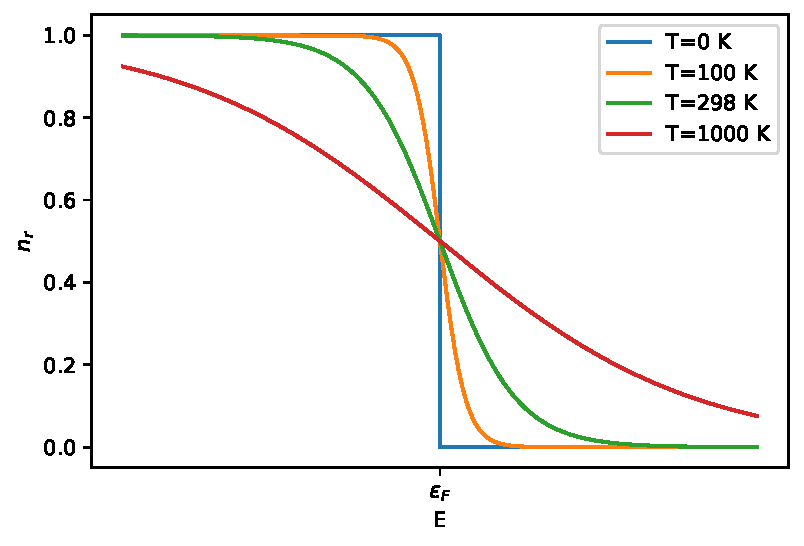
\includegraphics[scale=1]{03-Fermi-Dirac.pdf}
    \caption[short]{función de distribución de Fermi-Dirac}
    \label{Fig:3.2.01}
\end{figure}

Como sabemos, la densidad de estados (el número de estados entre $E$ y $E+\D E$) $g(E)$ de una partícula encerrada en un volumen $V$ es

\begin{equation}
\D \Omega (E) = g(E) \D E = (2S+1) \frac{4 \pi V}{h^3} (2m^3)^{1/2} E^{1/2} \D E
\end{equation}
donde $(2S+1)$ se debe a la degeneración debida al espín. Entonces el número de partículas con energías comprendidas entre $E$ y $E+\D E$ será $f_{FD}(E) \D E$, esto es, la \textbf{distribución de partículas de Fermi-Dirac}, tal que

\begin{equation}
f_{FD} = \bar{n} (E) g(E) = (2S+1) \frac{4 \pi V}{h^3} (2m^3)^{1/2} \frac{E^{1/2}}{e^{\beta(E-\mu)}+1}
\end{equation}
que es \textit{el número de estados posibles para esa energía por la ocupación media de dicho estado}. Una vez obtenida esta distribución de probabilidad anterior es trivial calcular la media de cualquier magnitud dada $\bar{A}$:

\begin{equation}
\bar{A} (E) = \int_0^\infty A(E) f_{FD} (E) \D E
\end{equation}
tal que:

\begin{equation}
\bar{A} (E) = \int_0^\infty A(E) f_{FD}(E) \D E
\end{equation}
Analicemos pues, la distribución de Fermi-Dirac para diferentes temperaturas. 
\begin{itemize}
\item Empecemos por $T=0$. En ese caso tenemos una distribución escalon, tal que

\begin{equation}
\bar{n}_r = \left\lbrace \begin{array}{ll}
1 & \ \varepsilon_r < \mu \\
0 & \ \varepsilon_r > \mu
\end{array} \right.
\end{equation}
¿Qué significa esto? Que a la temperatura $T=0$ todos los niveles de energía con menor energía que la energía de Fermi están ocupado, y todos aq	uellos con mayor energía están vacíos \textit{en cualquier instante}. Este hecho se debe a que, a la temperatura del cero absoluto, todas las partículas tienden a ocupar niveles con la menor energía posible. A mayores temperaturas, debido a las fluctuaciones térmicas, las partículas podrán excitarse ocupando niveles de energía mayores. Lógicamente para esta temperatura $\bar{n} (E) = 1$, por lo que:

\begin{equation}
\overline{N} (T) = \sum_r \bar{n}_r = \int_0^{\varepsilon_F} g(E) \D E = (2S+1) \frac{4\pi V}{h^3} (2m^3)^{1/2} \frac{2}{3} \varepsilon_F^{3/2}
\end{equation}
Deduciéndo así la expresión de la \textbf{energía de Fermi} de un gas de fermiones de $N$ partículas 

\begin{equation}
\varepsilon_F = \frac{h^2}{(\sqrt{2}(2S+1))^{2/3} 4m} \parentesis{\frac{3N}{\pi V}}^{2/3}
\end{equation}

\item Sea $T>0$. En ese caso lo más llamativo es que $\bar{n}_r(\varepsilon_r = \mu) = \frac{1}{2}$, de tal modo que los niveles con menor energía que $\varepsilon_F$  siempre verifican $\frac{1}{2}<\bar{n}_r$ y aquellos que tienen una energía superior $\frac{1}{2}>\bar{n}_r$.
\end{itemize}

\subsubsection{Bose-Einstein}

Los bosones, partículas de espín entero, no sufren las restricciones del principio de Pauli, por lo que el número máximo de bosones en el mismo estado es $n_{\max} = \infty$. En ese caso 

\begin{equation}
\Xi_{BE} = \prod_r \sum_{n_r=0}^\infty e^{-\beta (\varepsilon_r - \mu ) n_r}
\end{equation}
Que como podoemos ver es una serie geométrica de razón $e^{-\beta (\varepsilon_r-\mu)}$, que converge si y solo si $(\varepsilon_r - \mu)>0$. Esto significa que la función de partición de un gas bosónico únicamente está definida si el potencial químico del gas es menor que la energía de todos y cada uno de los estados cuánticos de partícula. Verificándose esta relación:

\begin{equation}
\Xi_{BE} = \prod_r \parentesis{\frac{1}{1-e^{-\beta (\varepsilon_r - \mu)}}}
\end{equation}
La obtención de los números medios ocupacionales puede calcularse por dos caminos diferentes, usando las mismas relaciones que antes. En este caso los números medios ocupacionales son:

\begin{equation}
\bar{n}_r = \frac{1}{e^{\beta (\varepsilon_r - \mu)} - 1}
\end{equation}
siendo esta expresión la conocida \textbf{distribución de Bose-Einstein}. La \textbf{distribución de partículas de Bose-Einstein}, tal que:

\begin{equation}
f_{BE}(E) \D E = (2S +1 ) \frac{4 \pi V}{h^3} (2m^3)^{1/2} \frac{E^{1/2}}{e^{\beta(E-\mu)}-1} \D E
\end{equation}

La representación gráfica de esta función \ref{Fig:3.2.02}.

\begin{figure}[h!]\centering
    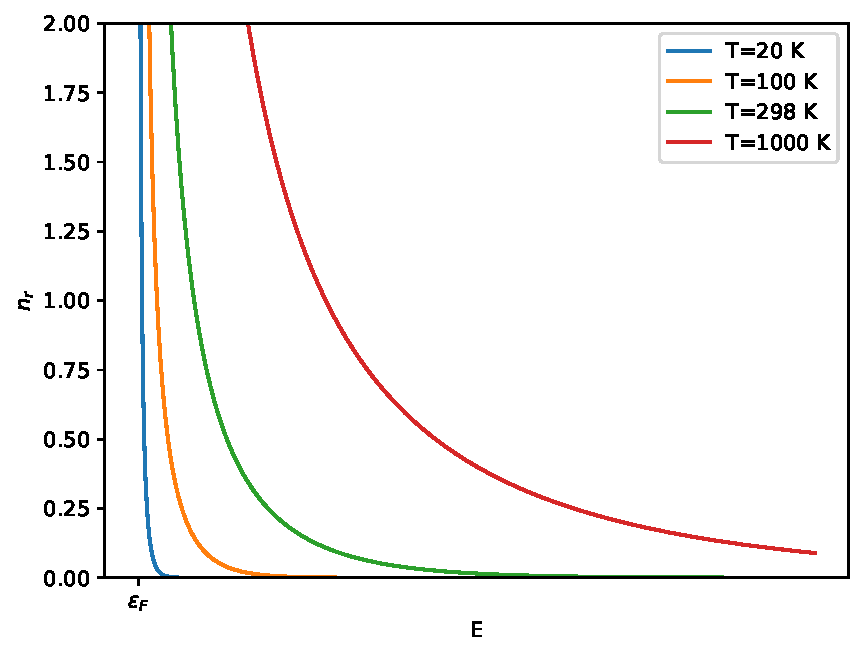
\includegraphics[scale=0.9]{03-Bose-Einstein.pdf}
    \caption[short]{función de distribución de Bose-Einstein}
    \label{Fig:3.2.02}
\end{figure}

\subsubsection{Maxwell-Boltzmann}

Examinemos ahora las estadísticas cuánticas en el límite en el que el número de ocupación sea mucho menor que uno, lo que tiene lugar cuando $e^{\beta (\varepsilon_r - \mu)} \gg 1$. Vamos a definir cuales son las condiciones de validez de esta aproximación:

\begin{itemize}
\item \textit{Bajas densidades y temperatura constante}.
\item \textit{Densidad fija y altas temperaturas}. 
\end{itemize}
En ese caso tenemos que podemos hacer la aproximación:

\begin{equation}
\bar{n}_r = e^{-\beta (\varepsilon_r - \mu)}
\end{equation}
A esta expresión se la conoce como la \textbf{distribución de Maxwell-Boltzmann}. Podemos expresar la ecuación \ref{Ec:3.2.007} como:

\begin{equation}
\ln \Xi_{MB} = \sum_r \ln \parentesis{\sum_{n_r=0} e^{- \beta (\varepsilon_r - \mu) n_r} }
\end{equation}
Si expresamos $\ln \Xi = \sum_r \ln \xi_r$, donde $\xi_r$ es la función de partición del estado $r$. En ese caso tenemos que

\begin{equation}
\ln \xi_r = \ln  \parentesis{ \sum_{n_r=0} e^{- \beta (\varepsilon_r - \mu) n_r}}
\end{equation}
Tanto para Fermi-Dirac  (recordemos que $\ln (1+x) \approx x$ si $x\ll 1$) como para Bose-Einstein (en este caso hay que aplicar además $1/(1-x) \approx 1+x$  si $x\ll 1$) el logaritmo puede expresarse como

\begin{equation}
\ln \xi_r \approx e^{- \beta (\varepsilon_r - \mu)}
\end{equation}
Podemos ver que si $z=\sum_r e^{-\beta \varepsilon_r}$ podemos expresar la función gran canónica como:

\begin{equation}
\ln \Xi_{MB}  = \sum_r e^{-\beta(\varepsilon_r - \mu)} = e^{\beta \mu} z
\end{equation}
Desarrollando esta exponencial en Taylor: 

\begin{equation}
\Xi_{MB} = \sum_{N=0}^\infty e^{\beta \mu N} \frac{z^N}{N!}
\end{equation}
Como podemos ver esto nos relaciona la \textit{función gran canónica Maxwell-Boltzmann} con la función canónica de un sistema de $N$ de partículas clásicas, indistinguibles e independientes:

\begin{equation}
Z_N = \frac{z^N }{N!}
\end{equation}


\newpage

\section{Gases ideales cuánticos}

En sistemas con dimensiones macroscópicas debemos hacer el paso al continuo, el cual se hace substituyendo sumas por integrales en el espacio de los momentos (espacio fásico), tal que

\begin{equation}
\sum_r \ \longrightarrow \frac{V}{(2\pi)^3} \int \D \kn  \equiv \frac{V}{h^3} \int \D \pn
\end{equation}
En el nuevo formalismo las magnitudes relevantes se hallan haciendo promedios integrales donde la función  $f(\epsilon)$ definida como

\begin{equation}
f(\epsilon) = \bar{n} (\epsilon) g(\epsilon)
\end{equation}
es la \textit{densidad de partículas con energías comprendidas entre $\epsilon$ y $\epsilon+\D \epsilon$}. Esta actuará como una auténtica función de densidad  de probabilidad en el espacio de energías. Así el valor medio de una magnitud cualquiera $A$ viene dada por:

\begin{equation}
\bar{A} = \int_0^\infty g(\epsilon) \bar{n} (\epsilon) A(\epsilon) \D \epsilon
\end{equation}
La gran función de partición para un gas de Fermi-Dirac (con +) o de Bose-Einstein (con -) viene dada por la ecuación:

\begin{equation}
\ln \Xi = \pm \int_0^{\infty}  g( \epsilon) \ln \ccorchetes{1 \pm e^{-\beta (\epsilon - \mu )}}   \D \epsilon
\end{equation}
Dado que este cálculo exige el conocimiento de la densidad de estados del sistema, lo que nos obliga a distinguir entre dos tipos de sistemas:

\begin{itemize}
\item \textbf{Gas no relativista:} la dispersión es $\epsilon = p^2 /2m$, por lo que la densidad de estados de partícula en una caja cúbida de lado $a$ (volumen $V=a^3$) será

\begin{equation}
\Gamma (E) = \frac{V}{6 \pi^2 \hbar^3} (2mE)^{3/2} \quad g(E) = g_s \frac{4 \pi V}{h^3} (2m^3)^{1/2} E^{1/2}
\end{equation}
donde $g_s=(2+1)$ es el factor debido al espín. \\

\item \textbf{Gas relativista}: la dispersión del gas de partículas de masa nula es $E=pc$ (no vamos a estudiar gases relativistas de masa no nula). De esto se puede deducir

\begin{equation}
\Gamma (E) = \frac{V}{6 \pi^2}  \parentesis{\frac{E}{\hbar c}}^3 \quad g(E) = \frac{V}{2 \pi^2 \hbar^3 c^3} E^2
\end{equation}
En el caso particular de fotones, las partículas tienen dos polarizaciones posibles (ondas transversales compatibles con las ecuaciones de Maxwell), por lo que la densidad de estados fotónica es:

\begin{equation}
g(E) = \frac{V}{\pi^2 \hbar^3 c^3} E^2
\end{equation}
\end{itemize}

Trataremos en primer lugar los gases no relativistas (electrones y bosones a bajas temperaturas) para terminar con el gas de fotones, intrínsecamente relativista. Llamemos al término $\lambda\equiv e^{\beta \mu}$ la \textbf{fugacidad}. En ese caso la integral a solucionar es:

\begin{equation}
\ln \Xi = \pm \frac{4 \pi V}{h^3} (2m^3)^{1/2} g_s \int_0^\infty e^{1/2} \ln (1\pm \lambda e^{-\beta \epsilon}) \D \epsilon
\end{equation}
Tenemos que las soluciones finales de la integral (para resolverla hay que desarrollar los logaritmos en función de su serie de Taylor). En ese caso tenemos que

\begin{equation}
\ln \Xi_{BE} = - g_s \ln (1- \lambda)+ g_s \parentesis{\frac{mk_B T}{2\pi \hbar^2}}^{3/2} g_{5/2} (\lambda)
\end{equation}
\begin{equation}
\ln \Xi_{FD} = g_s V \parentesis{\frac{mk_BT}{2\pi \hbar^2}}^{3/2} f_{5/2} (\lambda)
\end{equation}
donde hemos usado las funciones:

\begin{equation}
g_k (\lambda) = \sum_{n=1}^\infty \frac{\lambda^n}{n^k} \quad f_k (\lambda) = \sum_{n=1}^\infty (-1)^{n+1} \frac{\lambda^n}{n^k} 
\end{equation}
tal que $g_k(1)\equiv \zeta (k)$ la función \textit{Zeta de Riemann}. 

\subsection{Gas de bosones}

Usando la relación convencional de $\bar{N}$ como la derivada del logaritmo de la gran canónica respecto el potencial químico, tenemos que:

\begin{equation}
\bar{N} = \frac{g_s \lambda}{1-\lambda} + g_s V \parentesis{\frac{m k_B T}{2 \pi \hbar^2}}^{3/2} g_{3/2} (\lambda)
\end{equation}
Cuando $T=0$ tenemos que $\bar{N}=\bar{n}_0$ es el número medio de bosones en el estado fundamental, ya que como podemos comprobar

\begin{equation}
\bar{n}_0 = \frac{g_s \lambda}{1-\lambda} = \frac{g_s}{e^{-\beta \mu}-1}
\end{equation}
Que como podemos ver se anula cuando $\mu=0$. A la temperatura a la cual el potencial químico se anula se la conoce como \textbf{temperatura de Bose} $T_B$, y viene dada por:

\begin{equation}
T_B = \frac{2 \pi \hbar^2}{m k_B} \parentesis{\frac{\bar{N}}{g_{3/2} g_s V}}^{2/3}
\end{equation}
donde $g_{3/2}(1) = 2.616$. En muchas ocasiones veremos definida la \textit{longitud de onda térmica} $\lambda_T$:

\begin{equation}
\lambda_T \equiv \parentesis{\frac{2\pi \hbar^2}{mk_B T}}^{1/2}
\end{equation}
Luego, el número de bosones en el estado fundamental viene a $T<T_B$ muestra una dependencia de la temperatura como:

\begin{equation}
\frac{\bar{n}_0}{\bar{N}} = 1 - \parentesis{\frac{T}{T_B}}^{3/2}
\end{equation}
\subsection{Gas de electrones}

El gas de electrones se estudia para el caso particular $T=0$ para luego hacer un tratamiento heurístico para $T$ finita. Para la temperatura $T=0$ la densidad es q si $\epsilon_r \leq \mu$ y 0 si $\epsilon_r > \mu$. Así obteníamos la \textit{distribución del número de partículas Fermi-Dirac}:

\begin{equation}
f_{FD} = \left\lbrace \begin{array}{lr}
g(\epsilon) & \epsilon \leq \epsilon_F \\
0  \quad & \ \mathrm{resto}
\end{array} \right.
\end{equation}
Ya hemos calculado anteriormente la energía de Fermi, que es la que verifica que

\begin{equation}
N = \int_0^{\epsilon_F} g(\epsilon) \D \epsilon = g_s \frac{4 \pi V}{h^3} (2m^3)^{1/2} \int_0^{\epsilon_F} \epsilon^{1/2} \D \epsilon
\end{equation}
A partir de estas podemos calcular el momento de Fermi, la temperatura de Fermi y el vector de onda de Fermi. La energía media del gas de electrones viene dada por la ecuación:

\begin{equation}
\bar{E}_0 = \int_0^\infty g(\epsilon) \bar{n}(\epsilon) \epsilon \D \epsilon  = \frac{3}{5} \bar{N} \epsilon_F
\end{equation}
Veamos entonces que pasa cuando aumentamos la temperatura. En ese caso tenemso que la energía debe variar de tal modo que

\begin{equation}
\bar{E} (T) = \bar{E}_0 + k_B T \delta N
\end{equation}
donde $\delta N$ es el \textit{número de electrones en la franja de anchura $k_BT$} en torno a la energía de Fermi. Así:

\begin{equation}
\delta N \simeq g(\epsilon_F) k_B T = \frac{3}{2} \bar{N} \frac{T}{T_F}
\end{equation}
Luego, al orden más bajo de aproximación, la energía media del sistema será:

\begin{equation}
\bar{E} (T) = \bar{E}_0 + \frac{3}{2} k_B \bar{N} \frac{T^2}{T_B^2}
\end{equation}
A partir de la ecuación de la ecuación anterior es inmediato obtener la capacidad calorífica del gas de electrones:

\begin{equation}
C_v = \pparciales{\bar{E}}{T} \simeq 3 k_B \bar{N} \frac{T}{T_F}
\end{equation} 

\subsection{Gas de fotones}

El potencial químico de un gas de fotones debe ser nulo para que sea posible el equilibrio termodinámico del sistema. Luego, el número medio de fotones por estado cuántico de energía vendrá dado por la distribución de Bose-Einstein con $\mu=0$:

\begin{equation}
\bar{n} = \frac{1}{e^{\beta \epsilon}-1}
\end{equation}
Por lo que la densidad de fotones $f(\epsilon)=g(\epsilon)\bar{n}(\epsilon)$, viene dada por

\begin{equation}
f(\epsilon) = \frac{V}{\pi^2 \hbar^3 c^3} \frac{\epsilon^2}{e^{\beta \epsilon}-1} 
\end{equation}
Lógicamente podemos hacer el cambio de energía y frecuencia, de tal modo que $\epsilon = \hbar \omega$. 

\subsection{Gas de fonones}

En primera aproximación podemos ver un sólido como un conjunto ordenado de átomos, cada uno de ellos fijo en los nodos de una red que oscila en torno a su posición de equilibrio sometido a un potencial armónico. Los primeros intentos de calcular las propiedades termodinámicas de estos se hicieron desde la mecánica clásica, lo cual provocó fracasos estrepitosos, siendo incapaces de reproducir la capacidad calorífica de los sólidos a bajas temperaturas. No fue hasta Einstein y Debye, que demostraron que solo tratando cuánticamente un sólido podrían predecir correctamente los resultados experimentales. El modelo mas sencillo es el modelo de Eintstein, por lo que será tratado primero, para luego pasar al de Debye. Finalmente demostraremos que son equivalentes al gas de bosones con $\mu=0$.  

\subsubsection{Modelo de Einstein}

Einstein propuso la primera formulación teórica que permitió obtener un comportamiento cualitativamente correcto a bajas temperaturas, suponiendo que este está compuesto de $3N$  {\it osciladores armónicos unidimensionalmente, independientes y distinguibles}. El hamiltoniano de un oscilador armónico cuántico es: 

\begin{equation}
H = \parentesis{\hat{N}+ \frac{1}{2}}\hbar \omega
\end{equation}
donde $\hat{N}$ es el operador número. Su espectro de energía está dado por

\begin{equation}
\epsilon_n = \parentesis{n + \frac{1}{2}} \hbar \omega \quad n=0,1,2,...
\end{equation}
De este modo la \textbf{función de partición del modelo de Einstein} del sistema viene dado por: 

\begin{equation}
Z=\ccorchetes{\sum_{n=0}^{\infty} e^{-\beta \parentesis{n+\frac{1}{2} } \hbar \omega }}^{3N} 
\end{equation}
y su logaritmo neperiano (necesario para obtener la energía media, la entropía...) viene dado por

\begin{equation}
\ln (Z) = - 3N \ln \ccorchetes{2\sinh \parentesis{\frac{\beta \hbar \omega}{2}}}
\end{equation}

\subsubsection{Modelo de Debye}

Debye supone también que el sólido está compuesto por $3N$ osciladores armónicos, aunque incorpora al modelo de Einstein la existencia del acoplamiento entre los mismos. El hamiltoniano del sistema toma ahora la forma:

\begin{equation}
\hat{H} (\qn^N,\pn^N) = \sum_{i=0}^{3N} \frac{p_i^2}{2m} + \sum_{ij}^{3N} A_{ij} q_i q_j
\end{equation}
De esta manera queda codificada la información de las interacciones entre las partículas en la matriz $A_{ij}$, que puede diagonalizarse en las coordenadas $(Q_i,P_i)$. El resultado cuantizado del hamiltoniano es:

\begin{equation}
\hat{H} = \sum_{i=1}^{3N} \parentesis{\hat{N}_i+\frac{1}{2}} \hbar \omega_i; \quad N_i = a_i^+ a_i \quad \hat{N}_i |n_i \rangle = n_i |n_i \rangle
\end{equation}
Podemos interpretar entonces el conjunto de osciladores acoplados que forman el sólido en términos de unas cuasipartículas independientes denominadas \textbf{fonones} correspondientes a los modos colectivos del sistema que ocupan unos estados de energía $\epsilon_i = \hbar \omega_i$ definidos por los $3N$ modos normales del sistema. Los fonones u ondas sonoras corresponden en este modelo a las oscilaciones armónicas independientes de osciladores acoplados que forman el sólido. La función de partición canónica:

\begin{equation}
Z(T,V) = \prod_{i=1}^{3N} \sum_{n_i=0}^{\infty} e^{-\beta \hbar \parentesis{n_i + \frac{1}{2}}\omega_i}
\end{equation}
En cualquier caso la teoría de Debye \textit{considera el sólido un medio isótropo y continuo}, de tal modo que la relación a dispersión es $\omega  = k v$ siendo $v$ la velocidad del sonido. De esta relación es inmediato obtener la \textbf{densidad de estados del fonón}:

\begin{equation}
g(\omega) = \frac{V}{2\pi^2 v^3} \omega^2
\end{equation}
Para dos modos diferentes (dos modos transversales y un modo longitudinal), tenemos que

\begin{equation}
g(\omega) = \frac{V}{2\pi^2} \parentesis{\frac{2}{v_t^3} + \frac{1}{v_l^3}}\omega^2
\end{equation}
donde $v_t$ es la \textit{velocidad de propagación transversal} y $v_c$ la \textit{velocidad longitudinal}. Dado que tenemos un número máximo de estados de fonón por encontrarse en un sólido (a diferencia del gas de fotones) $N_{\max} = 3N$, implica que

\begin{equation}
3N = \int_{\Lambda} g(\omega) \D \omega  = \int_{\Lambda} \frac{V}{2\pi^2} \parentesis{\frac{2}{c_t^3} + \frac{1}{c_l^3}} \omega^2 \D \omega
\end{equation}
lo que nos lleva a que la región de integración $\Lambda$ debe estar acotado, por lo que existe una frecuencia máxima que se denomina \textbf{frecuencia de Debye} $\omega_D$. Esta debe venir dada por:

\begin{equation}
\omega_D^3 = \frac{18 N \pi^2}{V} \parentesis{\frac{2}{c_t^3}+\frac{1}{c_l^3}}^{-1}
\end{equation}
Los fonones son los cuantos del campo de ondas sonoras de un cuerpo macroscópico, y aparecen de manera totalmente análoga a los fotones en la cuantización del campo electromagnético. De la misma manera que en el caso de los fotones en una cavidad, estos son constantemente emitidos y absorbidos por la red, por lo que se verifica que $\mu=0$. 


\newpage

\section{Gas de Maxwell-Boltzmann}

Introduciremos en este capítulo el tratamiento de sistemas formados por partículas independientes y no localizadas en el límite clásico, esto es, con temperaturas y densidades ni extremadamente bajas ni extremadamente altas. Así podremos despreciar los efectos cuánticos derivados de la cuantización de la energía y de la indistiguibilidad de las partículas. Esto es lo que se denomina gas de Maxwell-Boltzmann, paradigma de la mecánica estadística. Comenzaremos el tratamiento de la termodinámica del gas ideal monoatómico (sin grados de libertad interno) en las diferentes colectividades, para luego introducir el gas diatómico. 

\subsection{Gas ideal monotatómico}

En el tema \ref{Sec:3} hemos visto que en el límite clásico $n_r \ll 1$ recuperamos la estadística de Maxwell-Boltzmann:

\begin{equation}
\bar{n}_r = e^{-\beta (\epsilon_r - \mu)}
\end{equation} 
Las condiciones de validez de la distribución de números medios de ocupación son equivalentes a la condición de validez de la descripción clásica de los microestados del sistema físico por lo que

\begin{equation}
\begin{array}{lll}
r & \rightarrow  &(\rn,\pn) \\ \\
\epsilon_r & \rightarrow  & H(\rn,\pn) \\  \\
\Gamma &  =  & \frac{1}{N!} \prod_{i=1}^N \frac{\D \rn_i \D \pn_i}{h^3} \\
\end{array}
\end{equation}
y consecuentemente las sumas de estados se vuelven una integral:

\begin{equation}
\sum_r \longrightarrow \int g(\epsilon) \D \epsilon ; \quad \int \frac{\D  \rn \D \pn}{h^3}
\end{equation}
Analizaremos en las secciones siguientes las propiedades termodinámicas del gas ideal de Maxwell-Boltzmann (gas ideal clásico) en las diferentes colectividades. \\

\subsubsection{Tratamiento microcanónico}

Consideremos un modelo de gas ideal monoatómico constituido por $N$ partículas independientes y por lo tanto puntuales aisladas en un volumen $V$. Supongamos que cada partícula tiene una masa $m$ y el sistema una energía $E$ constante (sistema aislado). En ese caso el hamiltoniano (no hay interacción) debe venir dado por

\begin{equation}
H (q,p) = \frac{1}{2m} \sum_{i=1}^N p^2_i
\end{equation}
La energía del sistema viene dada entonces por $E=H(p,q)$ ya que solo hay ligaduras holónomas (ligaduras del tipo $f(\zeta_1,\zeta_2,...)=0$ donde $\zeta_i$ es un grado de libertad o coordenada, como pueden ser $x$ o $p_y$). La obtención de la entropía del sistema (así como de otros valores medios) corre a cargo del volumen fásico/densidad de estados. Así, teniendo en cuenta que la hipersuperficie de energía constante $\sqrt{2mE}$ en el espacio de fases $3N$-dimensionales. Así el espacio de fases: 

\begin{equation}
\Gamma (E,V,N) = \int \cdots \int_{H\leq E} \D \Gamma
\end{equation}
donde, como de costumbre, el volumen fásico elemental viene cuantizado

\begin{equation}
\D \Gamma = \frac{1}{h^{3N}} 
\end{equation}
Por lo que en ese caso tenemos que:

\begin{equation}
\Gamma (E,V,N) = \frac{V^N}{h^{3N}} \int_{H\leq E}  \D \pn = \frac{V^N}{h^{3N}} \int p^{3N-1} \D p \D \Omega = \frac{V^N}{h^{3N}} (2m)^{3/2} \int \epsilon^{\frac{3}{2}N-1} \D \epsilon \D \Omega
\end{equation}
Como podemos ver dicha ecuación es la ecuación de un hipervolumen de radio $E^{3/2}$. Usando la ecuación del volumen de una hiperesfera de $f$ dimensiones

\begin{equation}
V_f = \frac{\pi^{f/2}}{(f/2)} R^f
\end{equation}
llegamos a que

\begin{equation}
\Gamma (E,V,N) = \frac{\pi^{3N/2}}{(3N/2)!} \frac{V^N}{h^{3N}} (2mE)^{3N/2}
\end{equation}
así la densidad de estados:

\begin{equation}
g(E) = \frac{\pi^{3N/2}}{(3N/2-1)!} \frac{V^N}{h^{3N}} (2m)^{3N/2} E^{3N/2-1}
\end{equation}
La densidad de estados es una función \textit{extremadamente creciente de la energía}, lo cual es una característica general de los \textit{sistemas normales}. \\

A partir del principio de Boltzmann ($S=\ln (\Gamma)$) podemos deducir sin problemas la entropía microcanónica de un gas ideal, ya que

\begin{equation}
S(E,V,N) = k_B \ln \Gamma (E,V,N) = k + \frac{3N}{2} \ln (E)
\end{equation}
doonde $k$ es una constante no dependiente de la energía (si del volumen y el número de partículas). Si quisiéramos recuperar el valor de la temperatura bastaría con:

\begin{equation}
\frac{1}{k_B T} = \pparciales{\ln \Gamma (E,V,N)  }{E}_{V,N} = \frac{3}{2} \frac{N}{E}
\end{equation}
Es decir:

\begin{equation}
E = \frac{3N}{2} k_B T
\end{equation}
Este enunciado está relacionado con el \textit{teorema de equipartición de la energía}, ya que como podemos ver cada grado de libertad lleva asociado $k_BT/2$ (hay $3N$ grados de libertad, 3 momentos por partícula). Otra variable que podemos calcular es la presión estadística $\bar{P}$:

\begin{equation}
\bar{P} = T \pparciales{S}{V}_{E,N} = \frac{k_B N T}{V}
\end{equation}
obteniendo la \textbf{ecuación térmica de estado} donde $Nk_B = nR$:

\begin{equation}
\bar{P} V = k_B N T
\end{equation}

\subsubsection{Paradoja de Gibbs: recuento correcto de Boltzmann}

Evidentemente la entropía obtenida a través  de la aplicación del \textit{principio de Boltzmann} debe verificar las mismas propiedades que la entropía termodinámica, esto es, que debe ser una magnitud extensiva (aditiva). Precisamente es base a la necesidad impuesta por el \textit{principio de aditividad de la entropía} se ha definido a la misma como una función logarítmica del número de microestados de entropía, ya que dos sistemas \textit{estadísticamente independientes} verifican que $\Gamma_{tot} = \Gamma_1 (E_1) \Gamma(E_2)$ lo que nos lleva a que

\begin{equation}
S_{tot} = S_1 + S_2
\end{equation}
Esta propiedad no puede destruirse por una modelización. Precisamente en esto consiste la {\it \textbf{paradoja de Gibbs}  para el gas ideal clásico}. Esto nos lleva a que el re-escalado de las variables extensivas, $X \rightarrow X' = \alpha X$ haga que la entropía también se re-escale de la misma manera $S' = \alpha S$. De no verificarse esto no se verificaría la propiedad de adicción de Boltzmann, incurriendo en la paradoja de Gibbs.  \\

Como sabemos de los temas anteriores, calcular el volumen fásico del sistema estadístico no es sino obtener el número de microestados del mismo compatibles con una energía dada $E$. Al realizar dicho contaje para el gas ideal clásico hemos incluido todas las posibles configuraciones de las $N$ partículas, pues hemos integrado a todo el volumen fásico sin exclusión alguna. Dado que no hemos contando las diferentes permutaciones, debemos corregir el \textit{volumen fásico}:

\begin{equation}
\Gamma ' = \frac{\Gamma}{N!}
\end{equation}
Como podemos ver la \textit{paradoja de Gibbs} marca los límites de la termodinámica clásica, obligándonos a introducir la indistiguibilidad de las partículas, propia de la mecánica cuántica, aún cuando en la mecánica clásica no se puede interpretar correctamente dicha innovación conceptual. 

\subsubsection{Tratamiento canónico}

El cálculo de la función de partición canónica del gas ideal en el límite clásico se reduce a la obtención de la función de partición individual de cada una de las partículas constituyentes del sistema. La estadística de Maxwell-Boltzmann canónica:

\begin{equation}
n_r = e^{-\beta (\epsilon-r - \mu) } \tquad \Xi_{MB} = \sum_{N=0}^\infty e^{\beta \mu N} Z_N
\end{equation}
donde 

\begin{equation}
Z_N = \frac{1}{N!} \ccorchetes{\sum_r e^{-\beta \varepsilon_r} }^N
\end{equation}
Dado que el límite clásico pasa de sumatorios a integrales:

\begin{equation}
Z_N = \frac{1}{N! h^{3N}} \int e^{-\beta \sum_i p_i^2 / 2m} \D \pn \D \qn = \frac{V^N}{N! h^{3N}} (2\pi m k_B T)^{3N/2} 
\end{equation}
(donde tenemos que integrar hasta el infinito, ya que ahora debido a las fluctuaciones térmicas todos los estados de momento son posibles). Podríamos haber llegado al mismo resultado empleando la función de partición de una partícula y elevando a $N$ (corrigiendo las permutaciones):

\begin{equation}
z_1 = \frac{1}{h^3} \int e^{- \beta p^2/2m}\D \pn \D \qn = \frac{V}{h^3} \parentesis{\frac{2 \pi m}{\beta}}^{3/2}
\end{equation}
A partir de esto podemos llegar a la \textbf{energía libre de Helmholtz}:

\begin{equation}
F = U -  TS = - k_B T \ln (Z_N) 
\end{equation}
A partir de la \textit{energía libre} podemos hallar todas las propiedades/relaciones termodinámicas de interés: 

\begin{itemize}
\item \textbf{Ecuación de estado calórica.} La expresión de la energía del sistema:

\begin{equation}
\bar{E} = - \pparciales{\ln(Z_N)}{\beta} = \frac{3}{2} N k_B T
\end{equation}
\item \textbf{Ecuación de estado térmica.} La presión de un colectivo estadístico se define a partir de las relaciones termodinámicas convencionales:

\begin{equation}
\bar{P}  = - \pparciales{F}{V}_{T,N} = k_B T = \frac{k_B N T}{V}
\end{equation}
llegando a la \textit{ecuación de Clapeyron} igual que en la colectividad microcanónica. \\

\item \textbf{Potencial Químico}. El potencial químico se puede deducir, a partir de la energía libre, como

\begin{equation}
\mu = \parentesis{F}{N}_{T,V} = - k_B T \ccorchetes{\ln \parentesis{\frac{V}{N}}  + \frac{3}{2} \ln \parentesis{\frac{3m\pi}{h^2}} - \frac{3}{2} \ln \beta }
\end{equation}
donde hemos usado la \textit{aproximación de Sterling}, de tal modo que

\begin{equation}
\mu = \mu^0 (T) + k_B T \ln \parentesis{\frac{V}{N}}
\end{equation}
\item \textbf{Entropía:} la entropía del sistema se define como $S=k_BT\ln F + \bar{E}/T$, de tal manera que 

\begin{equation}
S = k_B T \ccorchetes{\ln \parentesis{V}{N} + \frac{3}{2} \ln \parentesis{\frac{3m \pi}{h^2}}- \frac{3}{2} \ln \beta +1} + \frac{3Nk_B}{2}
\end{equation}
\end{itemize}

\subsubsection{Teorema de equipartición de la energía}

Aunque ya se ha introducido a lo largo de los temas anteriores el teorema de equipartición de la energía, es de la sede canónica donde podemos analizar con toda la generalidad posible dicho resultado. Consideremos un sistema descrito por un hamiltoniano $H(p^N,q^N)$ que puede descomponerse como

\begin{equation}
H = H'(q^N)  + \sum_{i=1}^N c_i p_i^2
\end{equation}
Entonces la energía media asociada al grado de libertad $p_i$ es de $\epsilon_i (p_i)=k_B T/2$. En base a este resultado, podemos formilar el teorema de equipartición:

\begin{theorem}[{\bf teorema de equipartición}]
Cada término cuadrático independiente del hamiltoniano contribuye al valor medio de la energía con $k_BT/2$.
\end{theorem}

Sin embargo es posible encontrar una versión más general de este teorema, el \textit{teorema de equipartición generalizado}, separado en dos teoremas, el de equipartición y el del virial. Sean $x_i$ y $x_j$ variables dinámicas sometidas a la condición de que $H$ sea $\infty$ en los extremos del intervalo de valores que toma $x_j$, se puede demostrar que

\begin{equation}
\left\langle x_i \parciales{H}{x_j} \right\rangle = k_B T \delta_{ij}
\end{equation}
de tal modo que podamos aplicarlo también a momentos y a posiciones. Así obtenemos:

\begin{itemize}
\item \textbf{Teoerema de equipartición.} En este caso las variables elegidas son momentos:

\begin{equation}
\langle p \ \partial_{p} H \rangle = k_B T
\end{equation}
\item \textbf{Teorema del virial.} Las variables elegidas son las posiciones generalizadas:

\begin{equation}
\langle q \ \partial_{q} H  \rangle = k_B T 
\end{equation}
\end{itemize}


\subsection{Gas ideal diatómico}

Consideremos ahora la termodinámica de un gas ideal formado por moléculas diatómicas. La principal diferencia con el caso tratado en las secciones anteriores es la existencia de grados de libertad internos asociados a los movimientos de rotación y de vibración de los núcleos que componen la molécula. El tratamiento general consistiría en escribir la ecuación de Schrödinger para los dos núcleos y los dos $n$ electrones y resolver esta ecuación obteniendo los autovalores y autovectores correspondientes, aunque la solución de este problema más allá de la molécula de $H_2$ es muy compleja. Por eso usaremos las aproximaciones correspondientes. \\

La \textbf{aproximación adiabática} o \textbf{aproximación de Born-Oppenheimer} es la hipótesis de que el movimiento nuclear y el electrónico en moléculas se pueden tratar independientemente. Esto es debido a que el movimiento electrónico es mucho más rápido que el nuclear de manera que los electrones se mueven en un campo generado por cargas nucleares esencialmente estáticas. En espectroscopia molecular esta aproximación consiste también en considerar la energía molecular como la suma de una serie de otras contribuciones independientes:

\begin{equation}
H = H_{espin \ nuclear} + H_{elec} + H_{vibr} + H_{rot} + H_{trasl}
\end{equation}
lo cual puede hacerse \textit{esencialmente porque los tiempos característicos (energías) son muy diferentes}. Otra aproximación muy válida (debido a sus bajos valores) es omitir el término del espín nuclear. Así la función de partición queda factorizada en 4 términos:

\begin{equation}
Z_N = \frac{z_1^N}{N!} \tquad z_1 = z_{trasl} z_{rot} z_{vib} z_{el}
\end{equation}
de acuerdo con lo anterior, el estado de movimiento se especifica mediante 6 grados de libertad, tres por cada núcleo. En general estos se especifican de la siguiente manera: 3 para el centro de masas, 2 para la rotación de la molécula y 1 para la libertad vibracional (distancia entre núcleos). Algunos de estos deben ser tratados cuánticamente, otros pueden aproximarse clásicamente. 

\begin{itemize}


\item El {\bf grado traslacional} es análoga al caso anterior para un gas ideal monoatómico, por lo que:
\begin{equation}
z_{trasl} = \frac{V}{h^3} \ccorchetes{\frac{2\pi(m_1+m_2)}{\beta}}^{3/2}
\end{equation}

\item La {\bf energía de rotación} vendrá dada por el hamiltoniano $H_{rot} = \frac{\Jn^2}{2I}$ donde $I$ es la constante de inercia (actúa como la masa para rotaciones rígidas). Así, usando los típicos autoestados $|J,,m_J\rangle$:
\begin{equation}
E_J = \frac{\hbar^2 J (J+1)}{2I} \quad J = 0,1,2\ldots
\end{equation} 
con una degeneración $g_J = 2J+1$. La distancia entre niveles energéticos suele estar entre \\

\begin{equation}
\Delta E = k_B \theta_{rot}
\end{equation}
donde $\theta_{rot} \sim 10 K$. Esto demanda un tratamiento cuántico, tal que

\begin{equation}
z_{rot} = \sum_{J=0}^{\infty} (2J+1) e^{- \frac{\theta_r J(J+1)}{T}}
\end{equation}
que puede hacerse continuo $J\rightarrow x$, de tal modo que:

\begin{equation}
z_{rot} \simeq \int_0^{\infty} (2x+1)e^{-\frac{\theta_r x(x+1)}{T}} \D x \simeq \frac{T}{\theta_r}
\end{equation}

\item Los {\bf grados vibracionales} necesitan un tratamiento cuántico debido a las elevadas energías entre estados. Así, recuperando el espectro de un oscilador armónico de frecuencia $\omega$:

\begin{equation}
z_{vib} = \sum_{n=0}^\infty e^{-\beta \parentesis{n+\frac{1}{2}}} = 
\frac{1}{e^{\beta \hbar \omega/2}-e^{-\beta \hbar \omega/2}} = \frac{1}{2\sinh \parentesis{\frac{\beta \hbar \omega}{2}}}
\end{equation}

\item Los grados de libertad electrónicos de la molécula viene dados por:

\begin{equation}
z_{el} = \sum_{n=0} e^{-\beta E_l}
\end{equation}
donde la suma se extiende a los estados electrónicos de la molécula. Los únicos niveles que contribuyen de manera efectiva a la función de partición son el estado fundamental y el primer estado excitado., lo que permite obtener la función de partición del gas ideal diatómico. 

\end{itemize}




\end{document}